\documentclass{beamer}
\usetheme{Dresden}
\usecolortheme{beaver}


\usepackage{fontspec}

\usepackage{natbib}

\title{Notes about clio}

\begin{document}

    \section{\cite{turchin_arise_2008}}

    \begin{frame}{What happen with the History? }
	\begin{itemize}
	    \item  No consensus (What explication is more plausible?)
		   \item  Too much theories and\ldots not enough understanding 
		   \item  Poor and limited data (fragmented sources)
		   \item  Necessity of an analytical and predictive history
	\end{itemize}
	\begin{center}
	    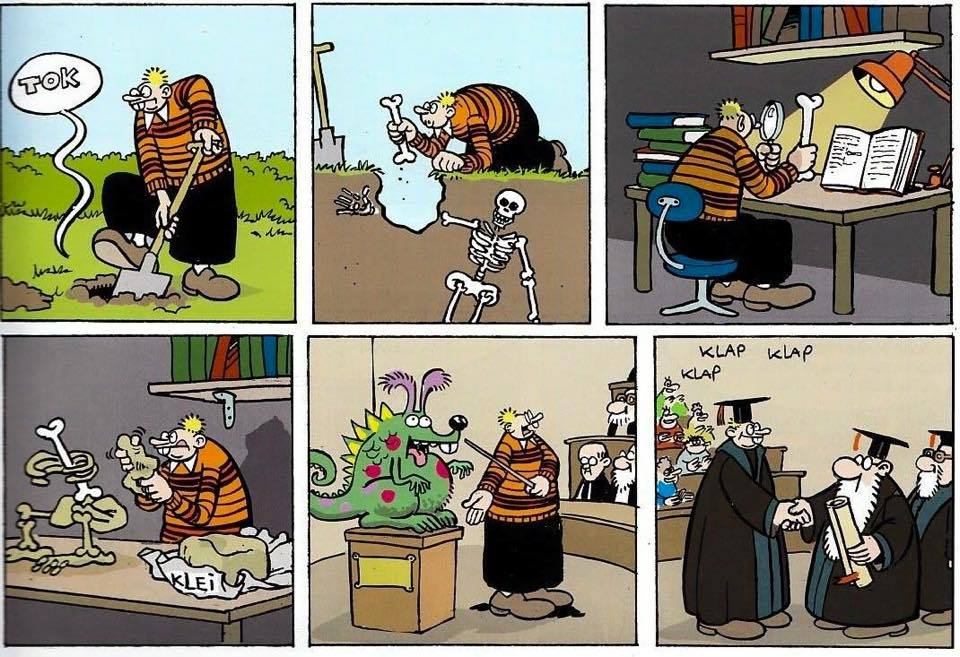
\includegraphics[width=6cm]{images/1}
	\end{center}
    \end{frame}

    \begin{frame}{		What did Turchin propose? }
	\begin{itemize}
	    \item Impossible to reform the historical approaches
		   \item New discipline
		   \item Necesity to apply analytical approaches to explain the past
		   \item Be more lumpers, my friend
	\end{itemize}
	\begin{center}
	    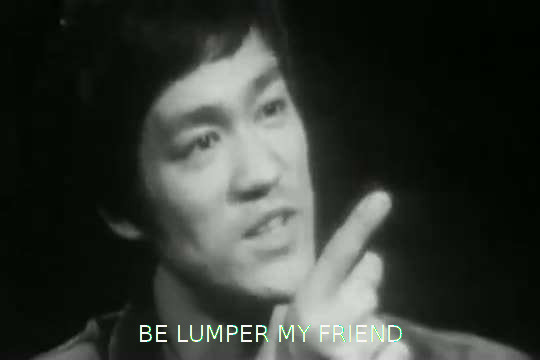
\includegraphics[width=4cm]{images/2.jpg}
	\end{center}
    \end{frame}

    \begin{frame}{Is it feasible? What will be our challenges? }

	\begin{itemize}
	    \item  Extremely complex to explain the human behaviour (unpredictable)
		   \item  Variability of social mechanisms
		   \item   Historical regularities can be studied (examples)
		   \item  Poor training of historians
	\end{itemize}
	\begin{center}
	    
\includegraphics[width=6cm]{images/3}
	\end{center}
    \end{frame}

    \begin{frame}{Cliodynamics? }
	\begin{itemize}

	    \item   Theoretical historical social science
		   \item   Dynamics are included to explain the varying processes 
		   \item   Unified theories using archaeological and history data (collected data)
		   \item   Idenfity patterns and natural laws in human behaviour (predictive)
	\end{itemize}

    \end{frame}

    \begin{frame}{Why Cliodynamics?}

	\begin{itemize}
	    \item  Posibility to become in a predictive science (searching the best data)
		   \item  Objectivity and Transdisciplinarity
		   \item  Test empirically all the collected data
		   \item  History must be transformed in a Science to be learned
	\end{itemize}
	\begin{center}
	    
\includegraphics[width=4cm]{images/3.jpg}
	\end{center}
    \end{frame}
    \begin{frame}{	Why NOT Cliodynamics? }

	\begin{itemize}
	    \item  Is it possible to create patterns? (freewill)
	    \item  Is it possible to change our way of working? (hypothesis.. what?)
	    \item  Physics envy?
	\end{itemize}

	\begin{center}
	    
\includegraphics[width=4cm]{images/5}
	\end{center}

    \end{frame}
\section{\cite{turchin_war_2013}}
\begin{frame}{One exemple of a ``Cliodynamic Study''}
    Recently, \cite{turchin_war_2013} developped the idea of Turchin in a article.
    We were lucky enough, Currie present it to us.
\end{frame}

\subsection{Historical Problem and Hypothesis }
\begin{frame}{Historical Problem and Hypotheses}
    \begin{block}{How human societies evolve from small group to huge society?}
	\begin{itemize}
	    \item Intense competition (Warfare) between society justify the use and maintain of costly institutions (ultrasocial norms and institutions, Turchin 2013).
	    \item Warfare depend on technological spread an geographic factors
	\end{itemize}
    \end{block}
\end{frame}

\subsection{Modelisation}
\begin{frame}{Why use a Model}
    ``Mathematical are important part of any mature science''(Turchin 2013, p 110):
    \begin{enumerate}
	\item Make assumption and mechanisms explicits \\
	    \rightarrow evaluation of the theories
	\item Quantitative prediction that can be tested against data \\ 
	    \rightarrow comparaison of alternatives hypotheses
    \end{enumerate}
\end{frame}

\begin{frame}{The Model}
     ``cultural evolution model'' that use ``Agent Based Modelisation''.
     Spatially distributed on Afroeurasian landmass on $100\times 100km$ squares
	 \begin{center}
	     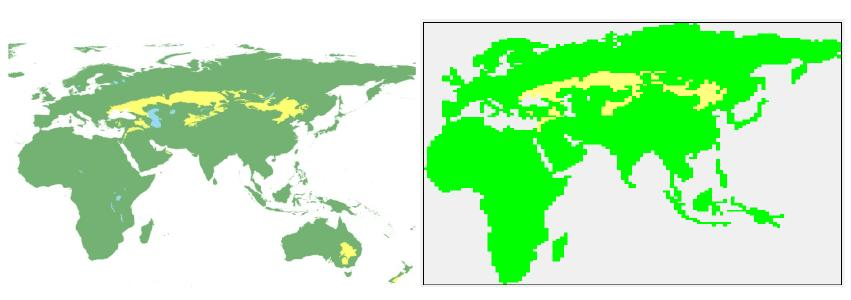
\includegraphics[width=6cm]{images/afroeurasian}
	 \end{center}
	 In each cell $\left\{
	     \begin{tabular}{@{}l@{}}
		     - agriculture or not \\
		     - biome (desert, steppe\ldots)\\
		     - elevation\\
		 \end{tabular}
	     \right.$
\end{frame}

\begin{frame}{Simulation}
    \begin{block}{Initialization}
	\begin{itemize}
	    \item Steppe cells : initialize military technology traits  (MilTech traits) that diffuse gradually.
	    \item Agricultural cells : communities with particular polity
	\end{itemize}
    \end{block}

	 community $\left\{
	     \begin{tabular}{@{}l@{}}
		 - $(x,y)$ coordinates\\
		 - $n_{ultra}$ ultrasocial traits ($U_{i,x,y}$)\\
		 - $m_{mil}$ MilTech traits ($M_{i,x,y}$) 
	     \end{tabular}
	     \right.$

\end{frame}

\begin{frame}{Critics}
    \cite{thomas_does_2014} critics of the previous article  (PNAS).

    One can notice that Thomas believe in the methods of Turchin but think that some choice are not good :
    
    \begin{enumerate}
	\item Abstraction problem (too abstract)
	\item Inovation process problem
	\item Fact that elevation $\uparrow$ defense
	\item random seeding alternativE
	\item too big (in term of time and space)
	\item no alternative causal pathway
    \end{enumerate}

\end{frame}

\begin{frame}{Answer to critics}
    \cite{turchin_reply_2014}: Answer to thomas (in PNAS but also in the Turchin's blog)
    \begin{itemize}
	\item Basically : Thomas didn't understand the paper
	\item Main arguments : it's the best way to do and the best hypothesis so far tested (do better and I will be happy).
    \end{itemize}
\end{frame}

\begin{frame}{General Critics}
    \begin{quote}
	``Turchin’s own example in the Nature article is really confined to uncovering a pattern, not testing an explanation.''\\
	Massimo Pigliucci
    \end{quote} 

\end{frame}


\begin{frame}
    \scriptsize
    \bibliographystyle{apalike}
    \bibliography{phd-journal-club}
\end{frame}
\end{document}

\begin{frame}{draft}
    \section{Notes abouts the Interview of turchin by Piglluci}
    is it possible to study history scientificly?
    are their general laws and principle underlying history?

    strong empirical patterns relation to Jared Diamond work on find general pattern
    but diamond got not go far, not bring the all power not quantitativ enough
    => objection good science field super string theories because it's impossible to test it
    history is easier to test than physical theory
    no science without empiracl test
    in principle string theory is testable
    in history it's easy

    prediciton is a step of scientific explenation and hypothesis testing.
    prediction in science is not about the future,

    detect cycle and test into other region and see if it happen

    Pigglucini : difference between detect pattern and speak about causal effect

    turchin vs malthus
    elite reproduction division of slice and vacante state


    After the black death in england and france both kingdom shoudl grow back under matlusian expection. But no. Unvaliadtion of the hypothesis.

    the black swan : how does unexpected event, which are those driving history, fit. => black swan : power law or pattern in any case.

    How much data? stochastic factor : statistics is mandatory.

    external vs internal factor:


    historian don't call them scientist, they called them Humanist.

\end{frame}
